\section{Shapes as Equivalence Classes}

\subsection{Motivating the Concept of Shape}
When we think about geometry, we often want to discuss ``shapes'' in $\mathbb{R}^n$. A first attempt at formalizing this concept is to say that a shape is simply a subset of $\mathbb{R}^n$.

For example, the circle of radius 1 centered at the origin in $\mathbb{R}^2$ can be defined as:
\[ C_0 = \{ (x, y) \in \mathbb{R}^2 \mid x^2 + y^2 = 1 \} \]

But here's a question: what about the circle of radius 1 centered at the point $(2, 1)$?
\[ C_{(2,1)} = \{ (x, y) \in \mathbb{R}^2 \mid (x-2)^2 + (y-1)^2 = 1 \} \]

Are these two different shapes? Intuitively, they are the \textit{same} shape—a circle of radius 1—just positioned at different locations. We don't want the location to matter when defining what a ``shape'' is.

\subsection{Congruence by Translation}
To formalize the idea that $C_0$ and $C_{(2,1)}$ are the ``same shape,'' we introduce the notion of \textbf{congruence by translation}.

Two subsets $K, L \subseteq \mathbb{R}^n$ are said to be \textbf{congruent by translation} (denoted $K \cong_T L$) if there exists a vector $y \in \mathbb{R}^n$ such that $K+y = L$.

This connects to high school geometry: two shapes are ``congruent'' if you can pick one up and place it on top of the other. In this context, we restrict to pure translation (no rotation).

\textbf{Example:} The two circles $C_0$ and $C_{(2,1)}$ are congruent by translation. Indeed, if we translate $C_0$ by the vector $y = (2, 1)$, we get:
\[ C_0 + (2,1) = \{ (a+2, b+1) \mid a^2 + b^2 = 1 \} = \{ (u, v) \mid (u-2)^2 + (v-1)^2 = 1 \} = C_{(2,1)} \]

\subsection{Shapes as Equivalence Classes of Sets}
Congruence by translation is an equivalence relation on the collection of subsets of $\mathbb{R}^n$.

\textbf{Exercise:} Verify that $\cong_T$ is reflexive, symmetric, and transitive. (Hint: Use properties of vector addition. This follows the same pattern as the arrow equivalence relation we prove in Section 3.6.)

To make congruent sets count as the \textit{same} shape, we define a \textbf{shape} to be an equivalence class under this relation. That is, a shape is not a specific subset of $\mathbb{R}^n$, but rather a collection of all subsets that are congruent by translation to one another.

Under this definition, the circles $C_0$ and $C_{(2,1)}$ belong to the same equivalence class, so they represent the same shape: ``a circle of radius 1.''

\subsection{Generalizing to Tuples of Points}
The concept of congruence by translation can be generalized in an obvious way to tuples of points or even to tuples of sets. For instance, two pairs of points $(x_1, x_2)$ and $(y_1, y_2)$ could be considered congruent if there exists a translation $v$ such that $x_1 + v = y_1$ and $x_2 + v = y_2$.

This generalization is particularly useful when we want to study geometric objects that are defined not just by a single set, but by relationships between multiple points or sets.

\subsection{Arrows: A Useful Special Case}
A particularly important application of this idea is to \textbf{arrows}. In high school physics or geometry, we often draw ``arrows'' to represent vectors. An arrow has a starting point and an ending point.

Consider two points $x, z \in \mathbb{R}^n$. We can draw an arrow starting at $x$ and ending at $z$. Intuitively, we say that the arrow from $x$ to $z$ represents the same vector as the arrow from $x'$ to $z'$ if they are parallel and have the same length.

Mathematically, we can formalize this using the concept of congruence: two pairs of points $(x, z)$ and $(x', z')$ should be considered equivalent (represent the same arrow) if there exists a translation that maps $x$ to $x'$ and simultaneously maps $z$ to $z'$. This happens precisely when $z - x = z' - x'$.

\subsection{Formal Definition: Arrow Equivalence}
We define a relation $\sim$ on the set of pairs of points $\mathbb{R}^n \times \mathbb{R}^n$.
We say that $(x, z) \sim (x', z')$ if:
\[ z - x = z' - x' \]

This is an \textbf{equivalence relation} (it is reflexive, symmetric, and transitive).

\begin{proof}
We verify the three properties of an equivalence relation:
\begin{itemize}
    \item \textbf{Reflexivity:} For any pair $(x, z)$, we have $z - x = z - x$, so $(x, z) \sim (x, z)$.
    
    \item \textbf{Symmetry:} If $(x, z) \sim (x', z')$, then $z - x = z' - x'$. This implies $z' - x' = z - x$, so $(x', z') \sim (x, z)$.
    
    \item \textbf{Transitivity:} Suppose $(x, z) \sim (x', z')$ and $(x', z') \sim (x'', z'')$. Then $z - x = z' - x'$ and $z' - x' = z'' - x''$. By transitivity of equality, $z - x = z'' - x''$, so $(x, z) \sim (x'', z'')$.
\end{itemize}
\end{proof}

\textbf{Geometric Intuition:} The condition $z - x = z' - x'$ is equivalent to saying $z' - z = x' - x$, meaning the quadrilateral formed by points $x, z, z', x'$ is a parallelogram. This visually shows that the arrows have the same direction and length.

\begin{center}
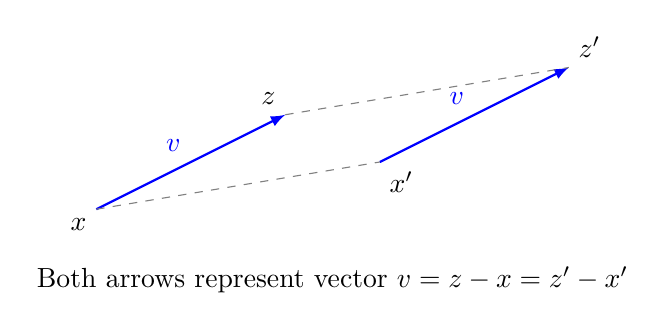
\begin{tikzpicture}[scale=1.2]
    % Define points
    \coordinate (x) at (0,0);
    \coordinate (z) at (2,1);
    \coordinate (xp) at (3,0.5);
    \coordinate (zp) at (5,1.5);
    
    % Draw arrows
    \draw[-latex, thick, blue] (x) -- (z) node[midway, above left] {$v$};
    \draw[-latex, thick, blue] (xp) -- (zp) node[midway, above left] {$v$};
    
    % Draw parallelogram
    \draw[dashed, gray] (x) -- (xp);
    \draw[dashed, gray] (z) -- (zp);
    
    % Label points
    \node[below left] at (x) {$x$};
    \node[above left] at (z) {$z$};
    \node[below right] at (xp) {$x'$};
    \node[above right] at (zp) {$z'$};
    
    % Show that both arrows represent the same vector
    \node[below] at (2.5, -0.5) {Both arrows represent vector $v = z - x = z' - x'$};
\end{tikzpicture}
\end{center}

We define an \textbf{arrow} to be an equivalence class under this relation.

\subsection{Representing Arrows}
An arrow (as an equivalence class of pairs of points) can be represented in two useful ways:

\textbf{1. As a vector in $\mathbb{R}^n$:} Each equivalence class corresponds to a unique displacement vector $v \in \mathbb{R}^n$. Specifically, the equivalence class of the pair $(0, v)$ contains all pairs $(x, z)$ such that $z-x = v-0 = v$. Thus, we can identify an arrow with the vector $v = z - x$ for any representative pair $(x, z)$ in its equivalence class.

\textbf{2. As a drawn arrow:} Each equivalence class can be visualized by drawing an actual arrow from any point $x$ to the point $z = x + v$. Different choices of starting point $x$ give different visual arrows, but they all represent the same equivalence class (the same ``abstract arrow'').

\subsection{Worked Example: Equivalent Arrows in \texorpdfstring{$\mathbb{R}^2$}{R2}}
Consider the following pairs of points in $\mathbb{R}^2$:
\begin{itemize}
    \item $(x_1, z_1) = ((1, 2), (4, 5))$
    \item $(x_2, z_2) = ((0, 0), (3, 3))$
    \item $(x_3, z_3) = ((-1, 1), (2, 4))$
\end{itemize}

We compute the displacement vectors:
\begin{align*}
z_1 - x_1 &= (4, 5) - (1, 2) = (3, 3) \\
z_2 - x_2 &= (3, 3) - (0, 0) = (3, 3) \\
z_3 - x_3 &= (2, 4) - (-1, 1) = (3, 3)
\end{align*}

Since all three pairs yield the same displacement vector $(3, 3)$, they all belong to the same equivalence class. They represent the same arrow, which can be identified with the vector $v = (3, 3)$, even though the actual drawn arrows start and end at different locations.
